\section{Infrastructure: Utilities}
\label{sec:utilclasses}

\subsection{Introduction}

The previous Infrastructure section described the data handling 
objects in the ESMF library. This section describes the lowest level
objects in the infrastructure layer, the utility classes.

\subsection{Design Goals and Considerations}

The goal of the utility layer is to present a uniform interface
for common system functions.  Each hardware architecture and
software system has different system libraries and methods
for accomplishing what are logically the same tasks.  Routines
in this layer must insulate user code from these variations so that it is
portable from system to system.

\subsection{Overview}

The utility classes have very little in common;
some are lightweight classes which maintain no internal state; 
others have state and exist for the lifetime of the application.  
Some run within a single process; others exist per processor and 
may communicate to other instantiations of itself on different processors.
But each system implements these functions differently, and it
is important to have a uniform set of interfaces which
is portable from machine to machine.
Another advantage of collecting these functions 
into a base-level utility set is to help avoid circular referencing.
In most cases they occupy the lowest level of the object hierarchy.

Methods provided by utility classes are available for use by  
all other classes in the ESMF library.  
Some of these methods will be called directly by user-supplied
code; others are intended to provide support for internal ESMF 
library code.

The {\tt Layout} class is used by any part of the library which needs
to decompose a task/problem/dataset into subsets.
The decomposition must allow for mapping certain subsets onto the
underlying machine model in a preferential way; e.g. keeping
vertical blocks of a 3D decomposition on processors which share
a memory pool.
It is required to interact with both the Processing Element lists
and the Machine Model in order to accomplish this preferential
decomposition.

The abstraction of a Processing Element andlist is a simple  between
the underlying hardware processor ID and the application's view
of how to address individual processors.  

The Machine Model encapsulates all information about the
hardware configuration, memory structure, and available
communications protocols and bandwith.  It furnishes this
information to other parts of the library which can
make decisions about partitioning or selection of algorithms
based on the amount and types of resources available.

The {\tt Basic Communication} routines provide a uniform interface to
the variety of interprocess communication mechanisms available
on different hardware platforms.  
The basic functions include methods to send
and receive data, such as scatter, gather, send, receive,
reduction methods such as sum, global min/max, and methods
to synchronize such as barrier. 

The {\tt Time Manager} provides all general purpose time methods, both
for computing time instants (dates and times) and time intervals
(the difference between 2 time instants).   It also supports 
setting and handling alarm events, either one-shot or repeating.
Supported calendars include Gregorian, Julian, no-leap, 360-day, 
generic, and no-calendar.
Time intervals can range from the very brief -- any rational fraction
of a second -- to geologic time scales.
The {\tt Time Manager} also allows the user to control the format of
time instants and intervals as they are returned.

Many parts of the library are required to maintain unique name
spaces for their objects.  The {\tt Registry} supplies methods
for defining name spaces and adding and querying names in those
spaces.  In general there is will be one {\tt Registry} object per
process, but if the namespace spans processes then {\tt Registry} 
objects will have to do global communication in order to verify names
are unique within the entire application.

The {\tt Error Handler} provides both uniform handling of errors and
a way for user code to select how errors will be handled.
An integer error code can be returned from the library to the
calling code, or the library can print an error message and exit.

The {\tt Log} manages the complexity of serializing diagnostic
messages produced by a multiprocess application.  It provides
methods for uniformly formatting the messages to facilitate
post-processing by filters and automated tools.

The {\tt Diagnostic} routines provide assistance with both performance
profiling and code debugging.  Timing routines support measurement
of both serial and parallel time intervals around certain sections
of code.  Debugging routines allow dynamic control over the level
of detail, enabling or disabling of different functional categories,
and assist with bit-level comparisons for debugging strategies which 
involve running a simulation under differing conditions and
comparing intermediate results.  These routines use methods from
the Time class for computing profile information, and from 
the Log class to collect and output results.

\subsection{Programming Model}
\label{sec:progmodel}

The ESMF programming model defines abstractions that expose
features of the computing environment to the user.  It must support the 
efficient utilization of system resources such as   
computing hardware, OS, and standard library or vendor-supplied 
software (e.g., MPI or other message-passing software, Posix threads, OMP),
and must present a reasonably simple interface to the application 
developer.  

ESMF abstracts the compute elements over which data and tasks may be
distributed into decomposition elements, or DEs, which
are essentially threads.  For MPP architectures in which there
is tyically one thread per process, the DE degenerates to a process.
Depending on the hardware system, ESMF threads will be to a limited 
extent compatible with user-defined threads.  The user will have 
the option to enable ESMF threading or not.  In the latter case, the
DE again degenerates to a process.

DEs are organized into topologies, such as a 2D grid, by the Layout 
class.  A user can define their own Layout, or a Layout can be 
constructed automatically in the process of creating a Distributed 
Grid.  

The Layout for both homogeneous and heterogeneous programming
strategies can be described compactly and precisely by a Layout 
tuple (Ltuple) of the form: \\
($D_{1}$, $D_{2}$, ... $D_{n}$), where $D_{n}$ is a representation of
each dimension in the layout.  \\
Each $D_{n}$ takes the form \\
$D_{n}$ = (<$R_{1}$>($N_{1}$,$C_{1}$), <$R_{2}$>($N_{2}$,$C_{2}$), ... <$R_{m}$>$(N_{m}$,$C_{m}$)<$P$>) \\
where \\
$R_{m}$ = number of repetitions \\
$N_{m}$ = number of DEs \\
$C_{m}$ = connectivity \\
$P$ = periodic boundary \\

Default values for connectivity are: \\
0 = unrelated processes \\
1 = adjacent processes, e.g. processes on the same node\\
2 = shared memory \\

Figure \ref{fig:layouts} shows number of examples of Layout objects,
together with their Ltuple description.

\begin{figure}

\label{fig:layouts}
\scalebox{0.7}{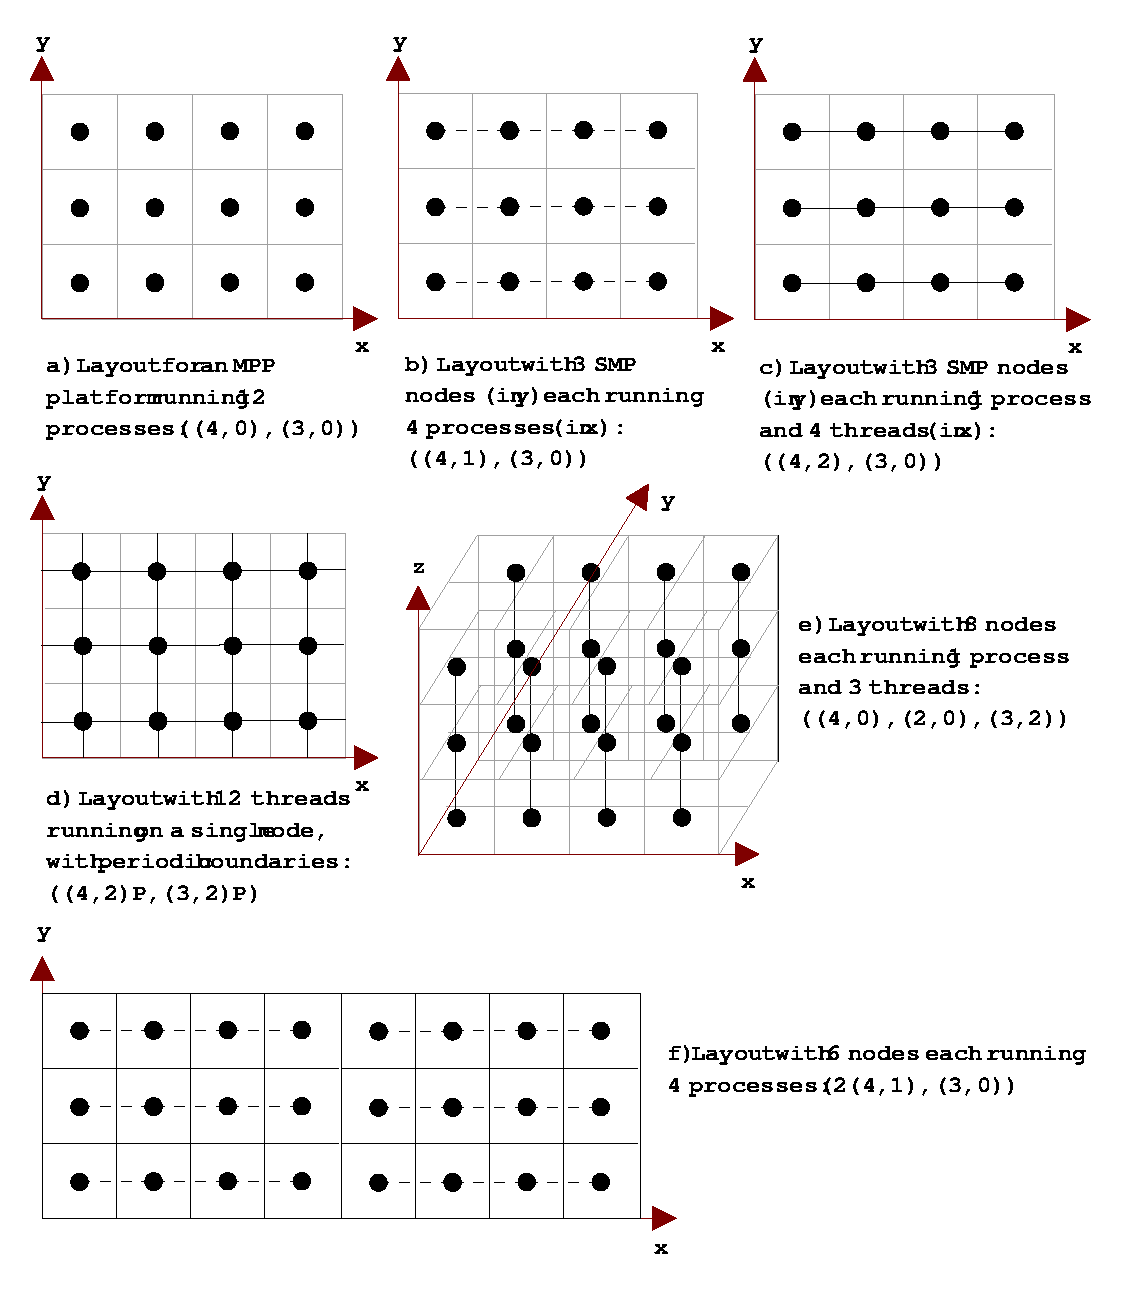
\includegraphics{Layout.eps}}
\end{figure}

When a {\tt Grid} object is defined on a {\tt Layout}, we require that the dimensions 
of the {\tt Grid} align with the dimensions of the {\tt Layout}.  The superimposition
of a {\tt Grid} on a {\tt Layout} is shown in Figure~\ref{fig:gridlayout}.

\begin{figure}
\label{fig:gridlayout}
\scalebox{0.7}{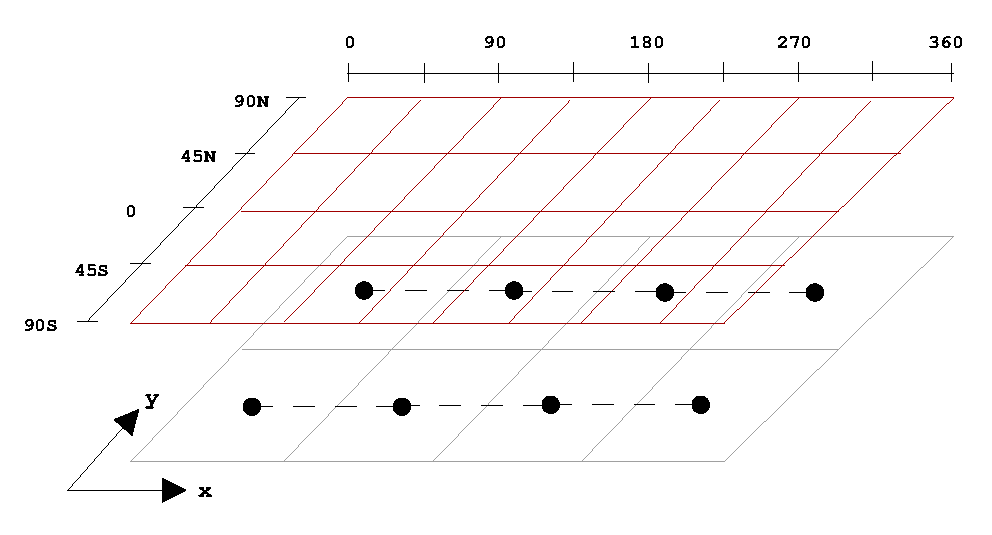
\includegraphics{GridLayout.eps}}
\end{figure}

The user can request system resources either through a simple processor
ID list, or by defining a {\tt Layout}.

\subsection{Class Details}

\subsubsection{Layout (ESMF\_Layout)}
\label{sec:layout} 
\begin{description}
\item [Description] A layout is a description of a computational domain that
may describe the decomposition of an Application, a Component, a Field Group, a Field, or 
a Distributed Grid.
If no Layout is specified for an object, it can inherit its layout from an object
higher in the data hierarchy.  
\item [Function] The Layout class maintains an N-dimensional set of decomposition
elements.  It provides methods for querying the set and requesting different
types of decompositions.  It maintains the mapping of tasks to decompositions.
\end{description}

\subsubsection{Processor Element list (ESMF\_PElist)}
\label{sec:pelist} 
\begin{description}
\item [Description] A Processor Element list is a list of physical processor IDs
available to participate in the computation.  
It includes a unique identifier for each PE which may differ from the
hardware processor ID, 
information about what memory or communication groupings it belongs to (e.g. subsets 
of PEs which share the same physical memory), 
and other identifiers for virtual resources.  
\item [Function] The PElist class encapsulates information needed to schedule
jobs in parallel, and is aggregated into the Layout class (see Section~\ref{layout}).
It provides query methods to the Layout object, and some limited query methods
may be available at the application level.
\end{description}

\subsubsection{Machine (ESMF\_Machine)} 
\label{sec:machine} 
\begin{description}
\item [Description] The Machine class provides a representation of 
key features of computer hardware and system software.  These
features include memory attributes and configuration, processor type and speed,
communication semantics and performance, 
interconnect attributes, and system library availability.
For the most part the application does not
interact directly with this class of object, although some 
user-level query routines may be provided.
\item [Function]
The purpose of the Machine is to store hardware and system software
information needed by the framework or application programmer in a general
form, but with little abstraction.  This information can be used to 
perform resource allocation, data distribution, and dynamic load balancing.  
The Machine can be queried for information such as
platform type(s), number of processors, number of threads, and number of 
nodes.  It will provide information on system library availability,
memory subsystem type (e.g. shared memory or not), 
communcation semantics, and optionally
may provide quantative information on actual bandwidth and 
latency through active tests.  
It is aggregated into the Layout class (see Section~\ref{layout}), and provides
methods for querying all characteristics needed by the Layout object to do 
problem decomposition and distribution of work.
\end{description}

\subsubsection{Basic Communications (ESMF\_BasicComm)}
\label{sec:basiccomm} 
\begin{description}
\item [Description] This library is a wrapper for MPI and other vendor-supplied 
message passing libraries.
\item [Function] The Basic Communication library provides a generic interface
and efficient communications for the ESMF.  Methods include scatter, gather, send,
receive, synchronize. 
\end{description}

\subsubsection{Time Manager (ESMF\_TimeMgr)}
\label{sec:timemgr} 
\begin{description}
\item [Description] The Time Manager provides time services to other objects
in the ESMF library and to application code.  It provides either absolute
time functions called Instants, or time differences called Intervals.
\item [Function] The Time Manager provides all general purpose time methods. 
It provides methods for supporting a variety of calendar time and dates,
for computing time intervals and instants from the very brief -- any 
rational fraction of a second -- to geologic time scales, and for
setting and handling alarm events, either one-time or repeating.
\end{description}

\subsubsection{Registry (ESMF\_Registry)}
\label{sec:registry} 
\begin{description}
\item [Description] A Registry maintains a list of (name, ID) pairs per 
namespace.  It supports the many classes in the system which are
required to have unique names, either per address space or over the entire
application.  
\item [Function] The Registry class supports multiple namespaces (e.g. per
field, per component, per exchange packet pool).  It provides methods to
create, query, and list namespaces and define their scope.  
Within a namespace it provides methods to
verify a name exists, add a (name, ID) pair if the name is unique,
generate a new unique name, retrieve an ID by name, and list existing names.
\end{description}

\subsubsection{Error Handler (ESMF\_Error)}
\label{sec:error} 
\begin{description}
\item [Description] The Error Handler allows the application to control 
the behavior of the library in case of error.  The library can return
control to the calling code with an integer error code and allow the
caller to handle the error.  An Error Print routine can
supply uniform text error messsage in addition to the integer error code.
Alternatively, the Error Handler can print an error message and exit.
\item [Function] The Error Handler class provides methods for selecting
the behavior of the library in case of error, methods to return uniform
text in addition to integer error codes, and methods to print the file
name, line number, and a description of the error before exiting the process.
\end{description}

\subsubsection{Log (ESMF\_Log)}
\label{sec:log} 
\begin{description}
\item [Description] The Log utility is intended to organize diagnostic
output, which may be generated in parallel at unpredictable times in
a multiprocessor environment.  It also attempts to organize
the diagnostic output so that searches and filters may be easily constructed. 
\item [Function] The Log class will be for diagnostic output. 
The bandwidth is assumed to be moderate to small, i.e. it will not be used 
to output large streams of numerical model output data.  
It provides methods for writing to the log, for specifying uniform
formatting information, for selecting a single unified log vs.\  a log 
file per processor.
\end{description}

\subsubsection{Diagnostics (ESMF\_Diag)}
\label{sec:diagnostics} 
\begin{description}
\item [Description] Diagnostics are collections of routines for
gathering information about how the simulation is behaving.  
These include both routines for finding program bugs
as well as understanding execution bottlenecks.
The Diagnostic class consists of two subclasses,
a Debug class for supporting methods for specifying
diagnostic information, and enabling and disabling the production of
that information.  The Performance class provides methods
for enabling and disabling timing routines in sections of
code, in both serial and parallel execution modes.
\end{description}




